\documentclass{article}

\title{Student Perceptions of Computing and Computing Majors\footnote{
\protectCopyright \copyright \confYear\ by the Consortium for Computing Sciences in Colleges.
Permission to copy without fee all or part of this material is granted provided
that the copies are not made or distributed for direct commercial advantage,
the CCSC copyright notice and the title of the publication and its date appear,
and notice is given that copying is by permission of the Consortium for
Computing Sciences in Colleges.  To copy otherwise, or to republish, requires
a fee and/or specific permission.
}}

\author{
Jeffrey A. Stone\\
Information Sciences and Technology\\
Pennsylvania State University\\
\email{stonej@psu.edu}\\
}

\begin{document}

\maketitle

\begin{abstract}
The growth in Computer Science (CS) program enrollments over the past decade, combined with an increased recognition of the importance of computing skills in the global economy, means that educational institutions have an opportunity to attract an increasingly diverse set of students. Despite robust enrollments, students may be entering university with misconceptions about computing, computing majors, and computing career prospects, potentially limiting long-term growth in computing programs. This paper updates the author’s previously published work by describing a study to elicit perceptions of computing and computing majors among a set of incoming students. The results suggest that while students have positive feelings towards computing, computing majors, and computing-related careers, significant differences exist for socioeconomic and gender groups.
\end{abstract}

\section{Introduction}
There has been a significant growth in undergraduate Computer Science (CS) program enrollments since 2006, with some estimates as high as almost 300\% growth \cite{roberts2018rising}. The increased recognition of computing and computational thinking as important skills \cite{grover2014remedying}, coupled with the needs of a growing job market, means that both primary and secondary level educational institutions have the opportunity and responsibility to construct curricula and recruitment plans that attract a diverse set of students. At the university level, incoming students are often perceived as “Digital Natives” who have been widely exposed to computing technology and are proficient in its use \cite{prensky2001digital}. Access to and use of computing technology is not uniform, however, and can differ based on socioeconomic status, gender, and other factors \cite{ritzhaupt2013differences}; such access and use can influence self-efficacy and academic success (\cite{hasan2003influence},\cite{jackson2008race}). As a result, initiatives to recruit a talented and diverse computing workforce are ongoing, ranging from primary school curricula development to policy advocacy (\cite{mcgill2016undergraduate}, \cite{scott2016broadening}).

While the positive growth in CS enrollments is encouraging, students may be entering university with misconceptions about the nature of computing, related majors, and related career prospects. These misconceptions are often thought to be formed from a variety of sociological and experiential factors, including K-12 experiences, demographic factors (e.g. gender, socioeconomic status), societal norms, and access to information technology. For example, prior research has suggested that students’ understanding of CS is often limited, perhaps due to insufficient career counseling and applications-centric high school computing curricula (\cite{egan2011impact},\cite{galpin2007perceptions}). Reported misconceptions of computing majors and careers have included social isolation, challenging curricula, and limited career options, among others (\cite{clarke1996characterizations},\cite{egan2011impact},\cite{yardi2007computing}). These misconceptions often lead to negative attitudes towards and a lack of awareness of computing majors \cite{grover2014remedying}, potentially limiting the ability of university computing programs to attract and retain students.

The goal of this study was to explore perceptions of computing and computing majors among a set of incoming university students by updating the author’s previous study \cite{stone2010factors}. The conceptual model for the study (Figure \ref{figure:model}) recognizes the relationship between a variety of social and academic influences – e.g. Information and Communications Technology (ICT) access and use, peers, parents, educators, K-12 education experience – and student perceptions of computing and computing majors, filtered through the lens of group differences (gender, race/ethnicity, and socioeconomic status). The research questions for this study were: \textit{What factors most influence students’ perceptions of computing and computing majors?} and \textit{What group differences exist in students’ perceptions of computing and computing majors?}

\begin{figure}[h]
\centering
\fbox{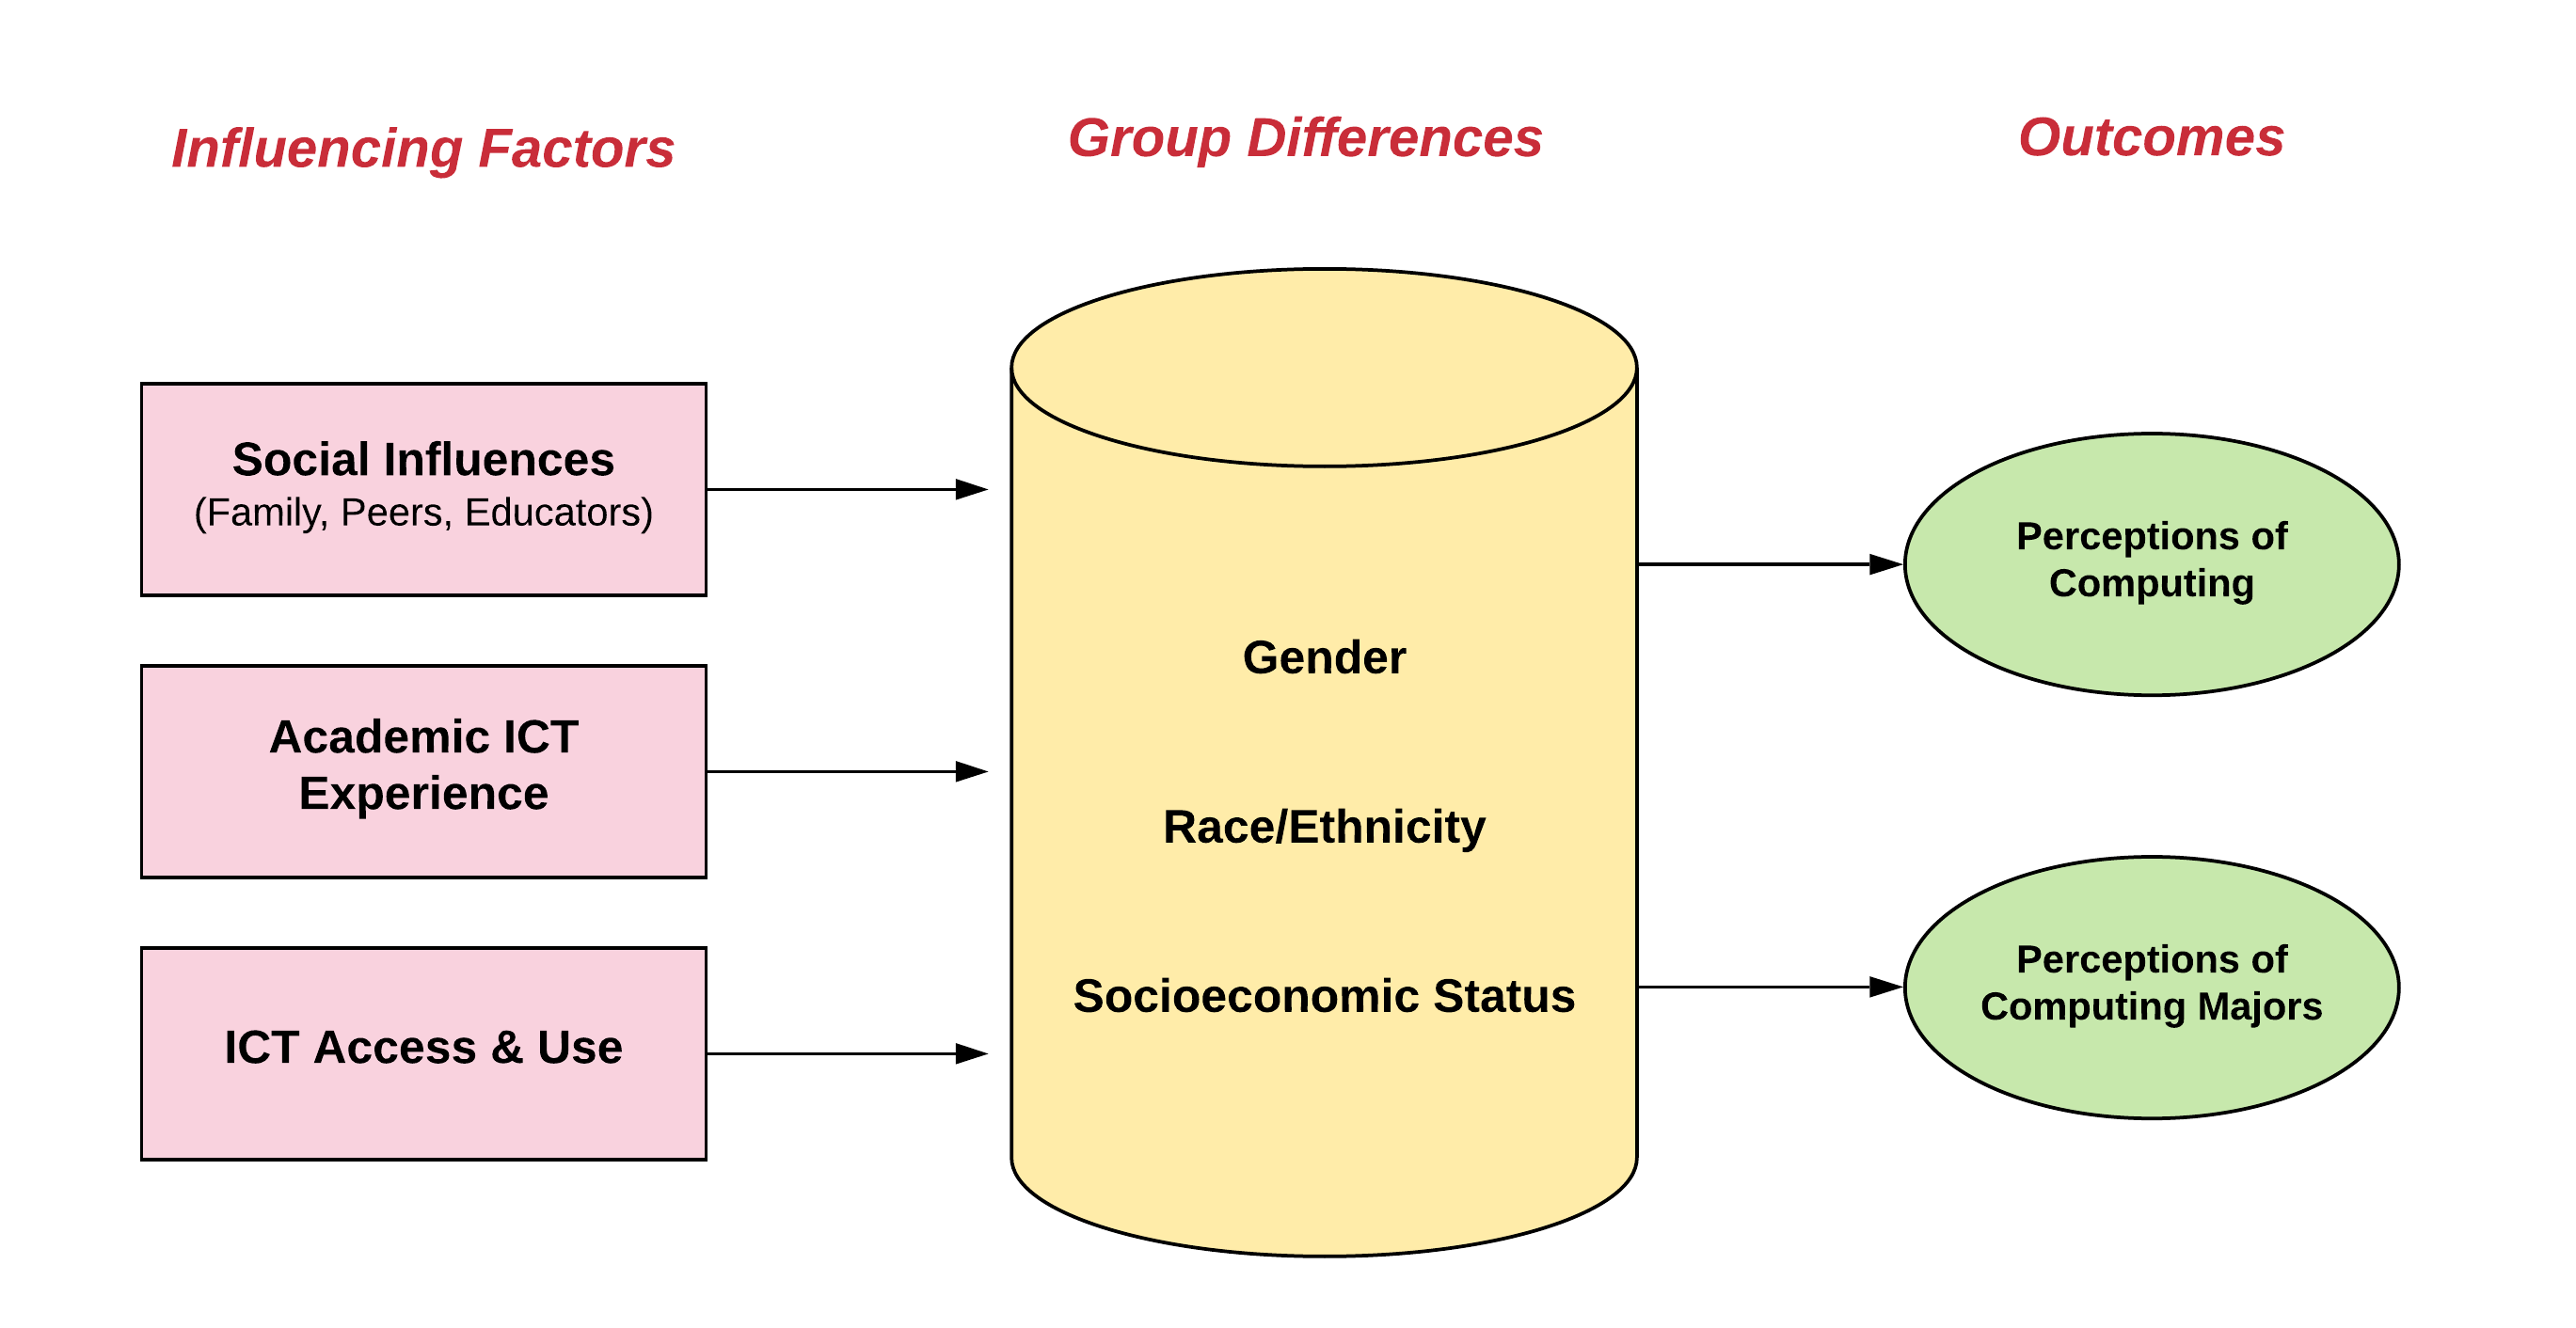
\includegraphics[scale=0.5]{195}}
\caption{Conceptual Model}
\label{figure:model}
\end{figure}

\section{Methodology}
An electronic survey was administered to a set of incoming students at one campus of a public research university during the 2017 summer orientation sessions. The survey was constructed based on prior research by the author \cite{stone2010factors} and a more recent literature review. Besides basic demographic questions, participants were primarily asked to respond to a series of Likert-style statements, using a five-level scale (1=Strongly Agree, 2=Agree, 3=Neutral [Undecided], 4=Disagree, and 5=Strongly Disagree). All research protocols and instruments were approved by the Penn State University Office of Research Protections.

\section{Survey Results}
A total of 161 students completed at least one question on the survey (78.54\%, \textit{N}=205). More than half the participants were female (55.33\%, \textit{n}=150). A majority of participants were 18-30 years old (97.33\%, \textit{n}=148) and White/Caucasian (76.00\%, \textit{n}=150). A majority of participants identified as commuters (62.00\%, \textit{n}=150) and were not considered first-generation college students (73.33\%, \textit{n}=150). In terms of community, 26.00\% (\textit{n}=150) came from a rural community, 31.33\% from suburbia, 40.00\% from an urban area (city/town), and 2.67\% were international students. Household income served as a proxy measure for socioeconomic status; a plurality of participants (45.83\%, \textit{n}=144) reported a household income of between \$50,000 and \$99,999, while a lesser amount reported household income less than \$50,000 (38.89\%). The following sections describe the survey results in light of the study constructs. Group differences are reported only when statistically significant.

\subsection{ICT Access, Use, and Academic Experience}
Participants most often reported using the Internet for more than 10 hours each week (60.00\%, \textit{n}=160), and most reported having Internet access at home (85.71\%, \textit{n}=161), at school (66.46\%), and via mobile devices (90.68\%). Most participants reported access to a computer in the home (86.34\%, \textit{n}=161) and at school (61.49\%). Access to tablet computers (e.g. Kindle, Galaxy, iPad) was uncommon; only 35.40\% reported having access to a tablet. Most participants reported using computers in high school (93.79\%, \textit{n}=161) and middle school (86.96\%). The most common high school computing course reported by participants was a Microsoft Office-style/basic computer skills course (72.67\%, \textit{n}=161). Other reported high school computing courses included graphic arts, digital photography, or digital video editing (32.92\%) and digital publishing (5.59\%). Only 13.04\% reported taking a computer programming course.

\subsection{Perceptions of Computing}
Most respondents agreed or strongly agreed with the statement \textit{Computer Technology improves our society} (69.81\%, \textit{n}=159). The importance of computing to respondents’ everyday lives was evident; a majority agreed or strongly agreed with the statement \textit{Computer Technology plays an important role in my everyday life} (77.36\%, \textit{n}=159) and with the statement \textit{Computer Technology plays an important role in the everyday life of my friends and family} (84.28\%, \textit{n}=159). Participants were also asked about the relationship of computing to their future careers. A majority of respondents agreed or strongly agreed with the statements \textit{Employers will expect me to have Computer Technology skills} (77.22\%, \textit{n}=158) and \textit{My future career will require me to use Computer Technology on a regular basis} (67.30\%, \textit{n}=159). Respondents overwhelmingly agreed or strongly agreed with the statement \textit{Computer Technology jobs will increase in the next 10-20 years} (86.79\%, \textit{n}=159). See Table \ref{table:comp}.
\begin{table}[h]
\caption{Perceptions of Computing Response Summary} % title of Table
\label{table:comp} % is used to refer this table in the text
\centering % used for centering table
\begin{tabular}{l c c c c } % centered columns (5 columns)
\hline\hline %inserts double horizontal lines
Statement & \textit{n} & Mean & Median & SD \\  % inserts table
%heading
\hline % inserts single horizontal line
Computing improves our society & 159 & 2.09 & 2.00 & 0.906 \\
Employers expect computing skills & 158 & 2.02 & 2.00 & 0.802 \\
My career will require computer use & 159 & 2.14 & 2.00 & 0.938 \\
Computing jobs will increase & 159 & 1.68 & 2.00 & 0.774 \\
Computing important in my life & 159 & 1.94 & 2.00 & 0.859 \\
Computing important for friends/family & 159 & 1.88 & 2.00 & 0.669 \\
\hline %inserts single line
\end{tabular}
\end{table}


Participants were asked to respond to the statement, \textit{How would you describe your feelings about Computer Technology?} with a five-level scale (1=Very Positive, 2=Positive, 3=Neutral (Undecided), 4=Negative, 5=Very Negative). A majority responded with very positive or positive feelings (71.07\%, \textit{n}=159). Significant differences between genders were found for this statement ($X^2$=9.73, df=4, p $<$ 0.05). Females had a higher mean response (2.33 vs. 1.90), meaning females were less likely to report positive feelings towards computer technology.

\subsection{Perceptions of Computing Majors}
A series of statements were used to determine the perceived value of computing majors and the prevalence of traditional stereotypes about computing. Over half the respondents agreed or strongly agreed with the statement Computing majors are difficult majors (51.57\%, \textit{n}=159), but recognition of the strong computing career prospects were seen in responses to the statement \textit{Students who are Computing majors are likely to have successful careers}. A majority (63.52\%, \textit{n}=159) agreed/strongly agreed with the statement. A note of positivity about computing majors (and diminishing stereotypes) was found in the percentage of disagree/strongly disagree responses to the statements \textit{Students who are Computing majors are more likely to be shy and non-social} (49.05\%, \textit{n}=159) and \textit{Computing majors and careers are primarily for male students} (66.04\%, \textit{n}=159). See Table \ref{table:compmaj}.

\begin{table}[h]
\caption{Perceptions of Computing Majors Response Summary} % title of Table
\label{table:compmaj} % is used to refer this table in the text
\centering % used for centering table
\begin{tabular}{l c c c c } % centered columns (5 columns)
\hline\hline %inserts double horizontal lines
Statement & \textit{n} & Mean & Median & SD \\  % inserts table
%heading
\hline % inserts single horizontal line
Computing majors are difficult majors & 159 & 2.50 & 2.00 & 0.745 \\
Students likely to be shy and non-social & 159 & 3.45 & 3.00 & 0.905 \\
Students likely to have successful careers & 159 & 2.26 & 2.00 & 0.750 \\
Computing primarily for male students & 159 & 3.76 & 4.00 & 0.984 \\
\hline %inserts single line
\end{tabular}
\end{table}


\subsection{Social Influences}
Two statements were used to assess the influence of parents and educators on the perceived importance of computing skills. A plurality of respondents agreed or strongly agreed (46.88\%, \textit{n}=160) with the statement \textit{My high school teachers and/or guidance counselors stressed the importance of Computer Technology Skills}. However, a plurality of respondents were undecided about the statement \textit{My parent(s) stressed the importance of Computer Technology Skills} (40.51\%, \textit{n}=158). Significant differences between the genders were found for this statement ($X^2$=10.82, df=8, p $<$ 0.05). Females were less likely to agree with the statement (M = 3.12 vs. M = 2.72). One-way ANOVA also found significant differences between responses to this statement and the reported household income (F[2, 139] = 3.34, p $<$ 0.05). Post-hoc Tukey analysis indicated that those respondents reporting a household income of less than \$50,000 (M= 3.16, p $<$ 0.05) were less likely to agree with the statement than those respondents reporting income in the [\$50,000-\$99,999] range (M = 2.72).

Three other statements were designed to assess the influence of parents and educators on students’ awareness of computing majors. A plurality of respondents agreed or strongly agreed with the statement \textit{My high school teachers and/or guidance counselors provided me with information on college-level Computing majors and careers} (41.25\%, \textit{n}=160). A plurality of respondents disagreed or strongly disagreed (38.99\%, \textit{n}=159) with the statement \textit{My parent(s) provided me with information on college-level Computing majors and careers}. One-way ANOVA found significant differences between responses to this statement and the reported household income (F[2, 140] = 5.79, p $<$ 0.01). Post-hoc Tukey analysis indicated that those respondents reporting a household income of less than \$50,000 (M = 3.43, p $<$ 0.01) were less likely to agree with the statement than those reporting income between \$50,000 and \$99,999 (M = 2.80). Finally, respondents were asked \textit{Who among the following people is the primary influence on your choice of major?} The majority reported that their choice of major was self-directed (70.44\%, \textit{n}=159), followed by family (17.61\%), friends (3.77\%), unknown (4.40\%), and teachers (1.89\%). See Table \ref{table:social}.

\begin{table}[h]
\caption{Social Influences Response Summary} % title of Table
\label{table:social} % is used to refer this table in the text
\centering % used for centering table
\begin{tabular}{l c c c c } % centered columns (5 columns)
\hline\hline %inserts double horizontal lines
Statement & \textit{n} & Mean & Median & SD \\  % inserts table
%heading
\hline % inserts single horizontal line
Teachers/counselors stressed skills & 160 & 2.61 & 3.00 & 0.991 \\
Teachers/counselors provided information & 160 & 2.91 & 3.00 & 1.103 \\
Parents stressed skills & 158 & 2.94 & 3.00 & 0.979 \\
Parents provided information & 159 & 3.16 & 3.00 & 1.071 \\
\hline %inserts single line
\end{tabular}
\end{table}

\section{Discussion and Conclusion}
The survey results show that these participants recognize the value of computing and computing majors, though it is unknown exactly how those perceptions are developed. As expected, computer and Internet access and use was very common among the study participants. Students are connected at school, at home, and on the go, and it plays a large role in their everyday lives and the lives of friends and family. Somewhat surprisingly, this does not translate into widespread enrollment in high school computing courses beyond simple MS Office-style applications courses. Enrollment in traditional CS-related high school courses (i.e. computer programming) was also very low.

The survey results also show that participants have a positive outlook on computing. Computing technology is seen as important to daily life, and respondents were very aware of the importance of computing skills for both their future careers and employment in general. A slight majority see computing majors as challenging; more importantly, existing stereotypes of computing students – shy, non-social, and male – are not considered reality among this population. However, the results involving parental and educator influence were surprising. While a plurality agreed that teachers and/or guidance counselors stressed the importance of computer skills, a minority of respondents indicated the same for parents. Males were much more likely to agree that parents stressed these skills. This gender disparity, coupled with the fact that females were significantly less likely to report positive feelings towards computing technology than males, raises concerns that gender-based disparities may persist. A minority of participants indicated that parents provided them with information on computing majors, while a plurality indicated that their teachers and/or guidance counselors did the same. Household income was a differentiator when it came to parental influence. Respondents with household incomes less than \$50,000 were less likely than respondents in the \$50,000-\$99,999 range to agree that parents provided them with information on computing majors or stressed the importance of computing skills. Universities should continue to provide outreach programs to attract and retain lower income and female students, though programs which can educate parents of these potential students about computing majors and careers should also be considered.

The study described in this paper provides some positive evidence that incoming students recognize the value and importance of computing, computing majors, and computing-related careers. The results are limited to a single university, but provide a basis for further exploration of both computing-related perceptions and the factors which may influence their development. The significant growth in CS program enrollments and the bright future for computing-related jobs provides universities with an opportunity to attract (and retain) an increasingly diverse set of students. By understanding some of the perceptions students have about computing, decision-makers can make more informed decisions about program offerings, marketing approaches, and retention strategies.

\section{Acknowledgements}
The author wishes to thank Bryan Valentine, Director of Student Affairs and Enrollment Services at Penn State Schuylkill, and Michael Koharcheck, undergraduate student, for their assistance in this project.
\medskip

\bibliographystyle{acm}
\bibliography{195}

\end{document}
